\section{Power Law Distribution Dataset}

\subsection{Part A: Developing Hypotheses}
Identify and collect a real-world dataset that you hypothesize follows a Power Law distribution. Please be clear about the reasoning behind your hypothesis and be specific about the source of the dataset.

For the Power Law distribution, we decided to select a well-known example of power lar in the real-world: a dataset of US city populations, sourced from this \hyperlink{https://www.kaggle.com/datasets/bharxhav/us-city-populations-and-coordinates}{Kaggle dataset}. The Power Law distribution captures a very unique proclivity of certain phenomenon to have extreme values you can count on being present; a notion predictable frequency of extreme values in the distribution. It still decays and extreme values do become more and more scarce further from the mean, however the Power Law distribution maintains some amount of mass it relies on to capture a predicatable extreme behavior in the data. In this context, we hypothesize that the population of cities will follow this distribution because although it is true that very generally larger cities become less commonplace as that population grows, however there always will be a small yet reliable amount of cities that are extremely large in size.\\

This behavior of city population is reflected in the PDF for Power Law:
$$
f(x) = \frac{\alpha - 1}{x_{\min}} \left(\frac{x}{x_{\min}}\right)^{-\alpha}
$$
the chance of observing a city with some input size is proportional to $ x^-a $, which dictates the natural inequality in the distribution between the average case behavior represented in the data and the extreme cases. This would allow the model to represent the proclivity of US cities to become mega-cities.\\

Regarding the data itself, it is a 2022 census of 19,268 US cities. For the purpose of fitting the Power Law model, it was necessary to remove 49 cities from the dataset that were made up of less than 10 people. This choice was made primarily because Power Law is designed to describe scaling behaviors about some minimum size, and in calculating logs of populations this small, we faced programmatic errors. Not to mention the census of cities this small could reflect some level of data collection error surely if the cities being characterized is the size of one large family. For this reason, and to preserve the underlying mechanism of the Power Law distribution, these "cities" were excluded.\\

\newpage
\subsection{Part B: Fitting Distributions}
For this exercise, we will call each of the four different theoretical distributions (normal, uniform, power law, exponential) a ``model". Fit the dataset (i.e., estimate the model parameters) against each model (not just the one you hypothesized) using maximum likelihood estimation (or using any technique you think is appropriate; make sure to comment on the validity of your approach). This should result in a total of \textbf{4 parameter sets}. Report the estimated parameters in the following tabular format:

\begin{center}
\begin{tabular}{|c|c|c|c|c|c|}
\hline
& & \multicolumn{4}{c|}{{\bf{\em{Model}}}}\\
\hline
{{\bf{\em{Dataset}}}} & {\bf{\em{\# Observations}}} &\textbf{Normal}& \textbf{Uniform} & \textbf{Power law} & \textbf{Exponential} \\
\hline
\textbf{Dataset 3} & $n_3$ & $\mu_3, \sigma_3$ & $a_3, b_3$ & $\alpha_3, x_{\min_3}$ & $\lambda_3$ \\
\hline
\end{tabular}
\end{center}

Be sure to show the code you used to arrive at your final estimates clearly.\\
-----\\
Below are the tabulated parameter estimates for this dataset (for the full tabulation described in the original assignment TeX, see Appendix). The code in Fig. 1 was also used to arrive at our final parameter estimates for this dataset, here is the same implementation below for convenience:\\
\begin{verbatim}
def dists_fit(input_csv: str) -> tuple:
    """
    Fits the obs dataset to each model using MLE.

    :param input_csv: Path to input data to fit paramater(s) to
    :type input_csv: str
    """
    obs = pd.read_csv(input_csv).iloc[:, 0].to_numpy()

    mu = np.mean(obs)
    std = np.sqrt(np.sum((obs - mu) ** 2) / len(obs))

    a, b = obs.min(), obs.max()

    alpha = 1 + len(obs) / np.sum(np.log(obs / a))

    lamb = 1 / np.mean(obs)

    return (mu, std, a, b, alpha, lamb)
\end{verbatim}

\vspace{4pt}

\begin{center}
\begin{tabular}{|c|c|c|c|c|c|}
\hline
& & \multicolumn{4}{c|}{{\bf{\em{Model}}}}\\
\hline
{{\bf{\em{Dataset}}}} & {\bf{\em{\# Observations}}} &\textbf{Normal}& \textbf{Uniform} & \textbf{Power law} & \textbf{Exponential} \\
\hline
\textbf{US City Populations} & 19268 & 10800, 83590 & 11, 8335897 & 1.206, 11 & 0.0000926 \\
\hline
\end{tabular}
\end{center}

\begin{center}
\textbf{Figure 10:} Parameter estimates for each model on US City Populations dataset.
\end{center}
\newpage

\subsection{Part C: Comparing Real and Synthetic Data}

For each fitted distribution (there will be 4 of them for this dataset, each corresponding to a different model), generate a synthetic sample of data points equal to the sample size of the real dataset using the respective model parameters you inferred from the real dataset.\\

Compare the real vs. synthetic data distributions using methods you think are the most appropriate, including visualizations. So, for this dataset, we compare the original dataset to four synthetic datasets, all with equal number of observations, but each synthetic dataset is generated using a different model.\\

For this dataset, identify the synthetic dataset (which corresponds to a model) that is most similar to the original data in terms of its distribution.\\

Now revisit your initial hypothesis. For this dataset: Did the dataset behave as expected, or was another model (assumed distribution) a better fit to the dataset? Reflect on why the observed results may differ from your expectations.\\
-----\\
We plotted a log-log Q-Q plot for the sample because of the magnitude of the sample ranges, which should in turn tell us which samples better resemble a Power Law distribution based on which are best aligned with the diagonal:

\begin{center}
  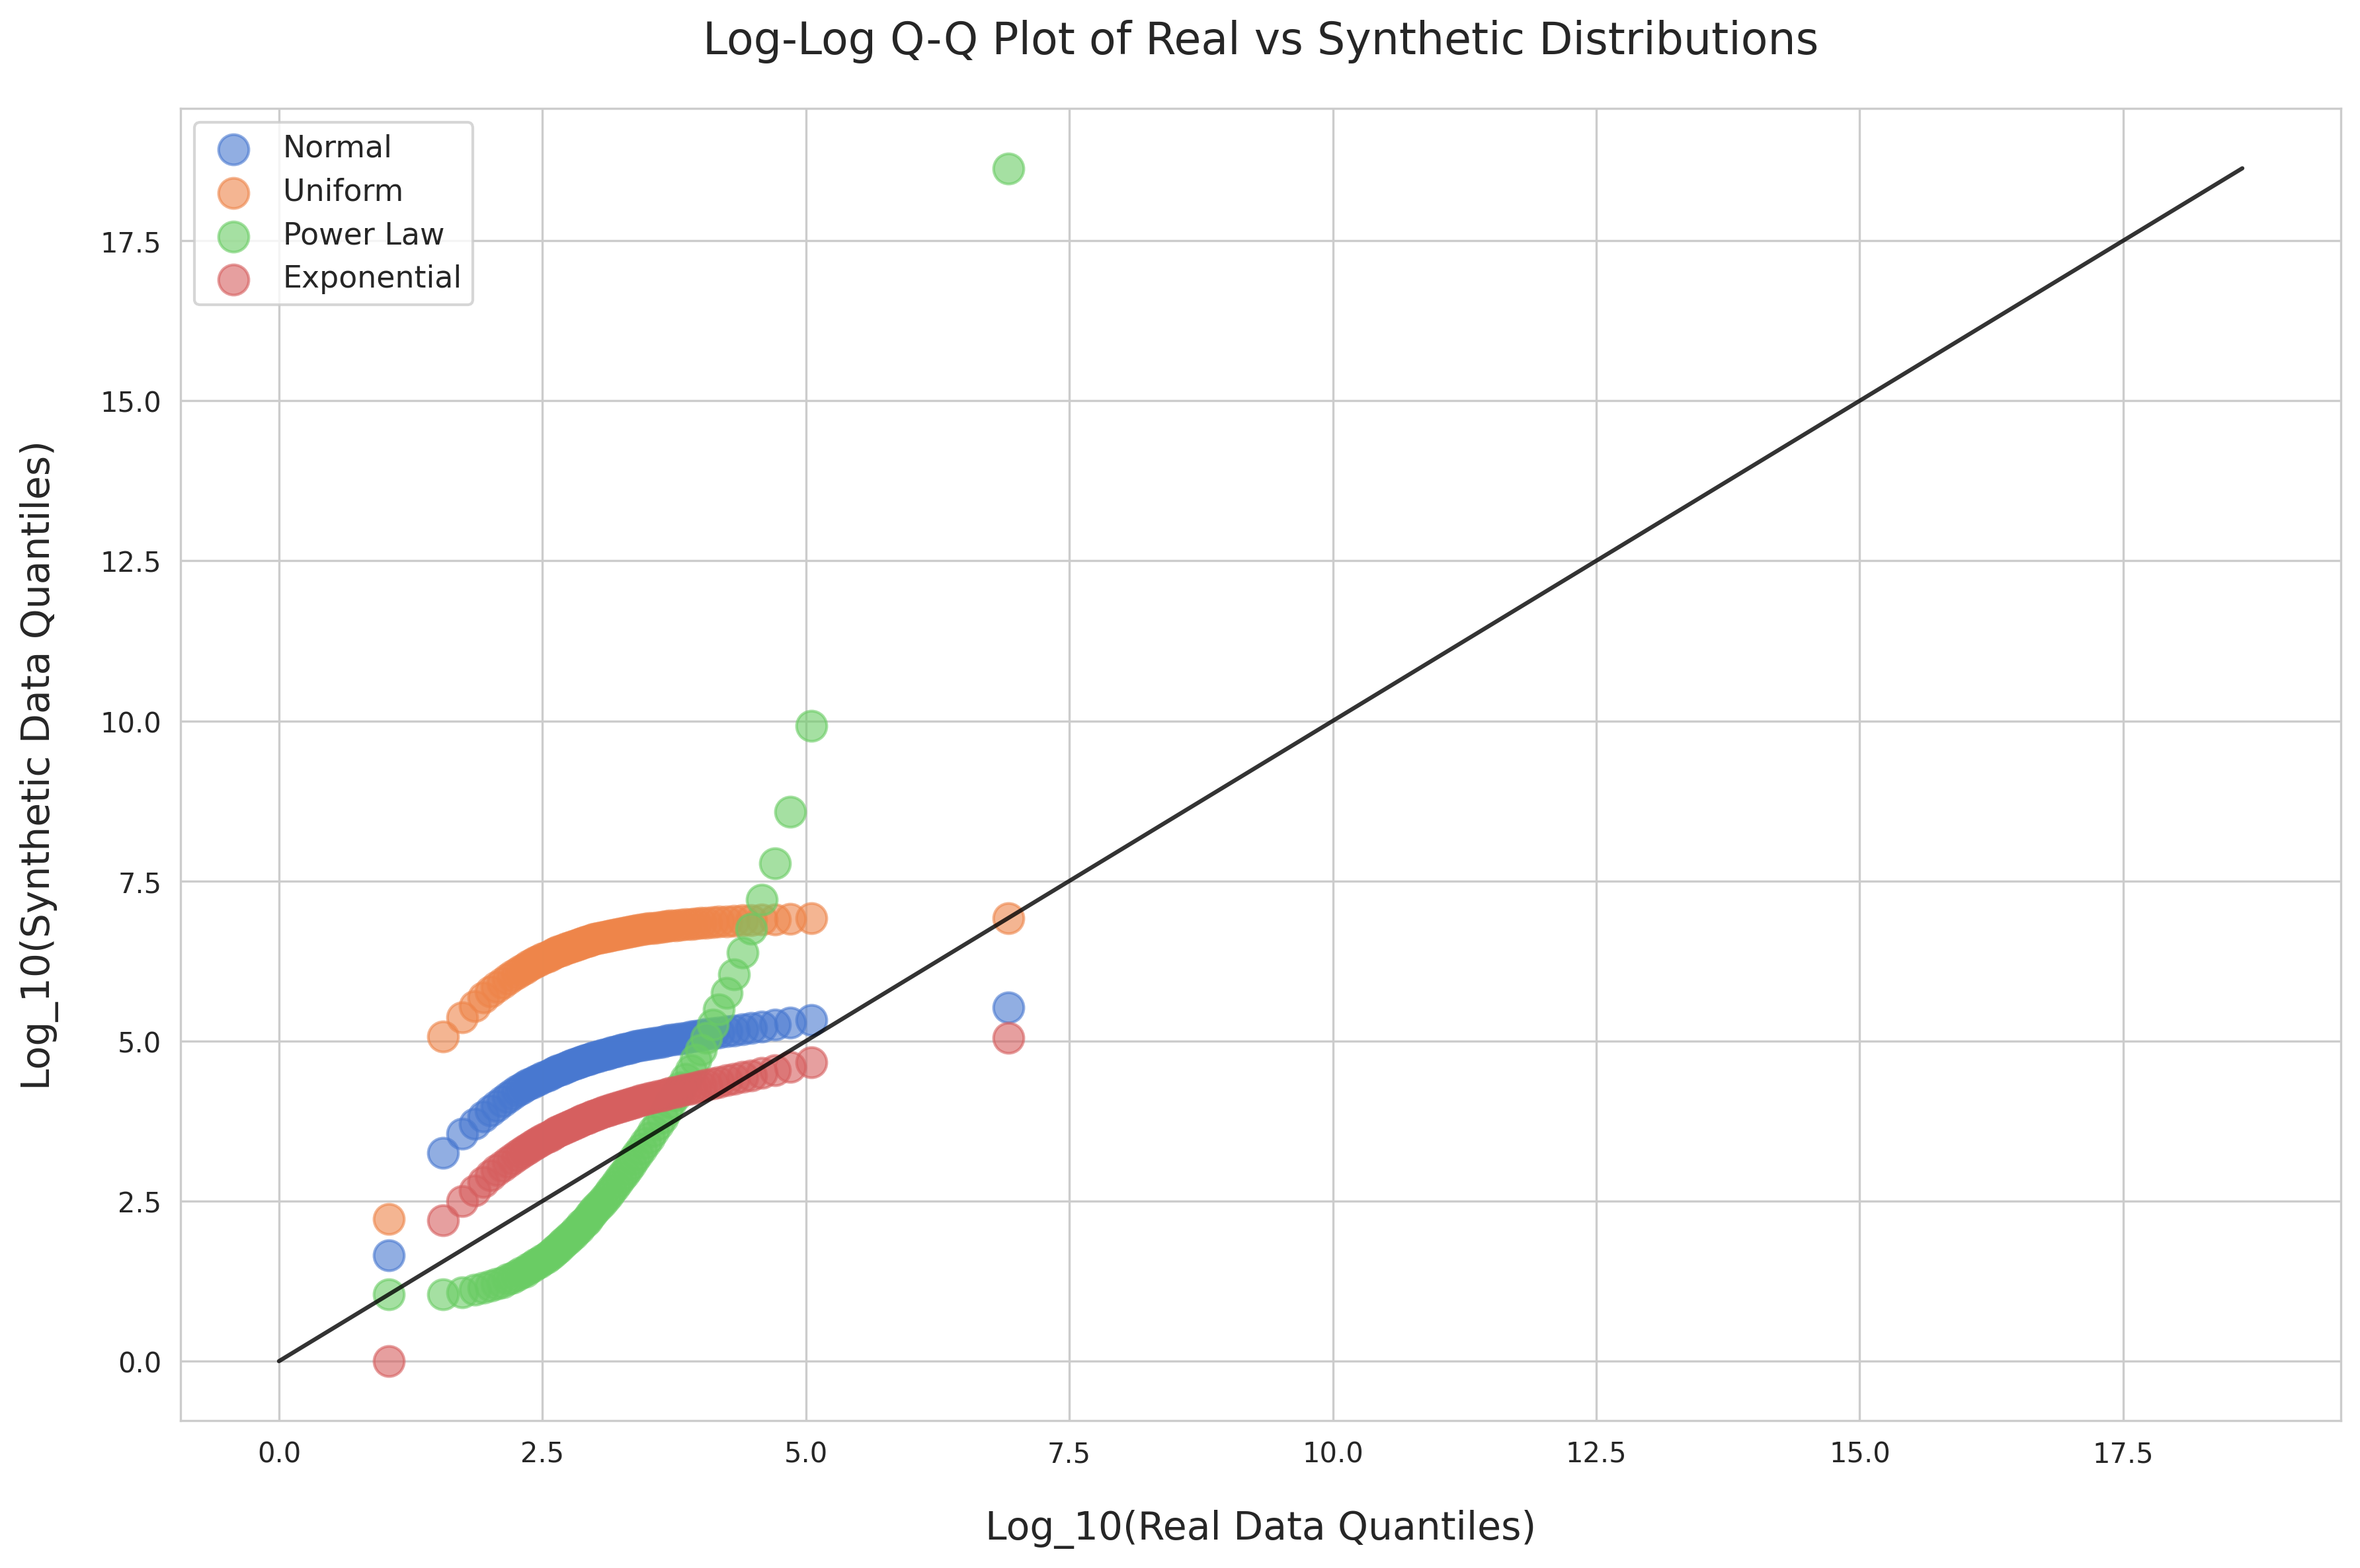
\includegraphics[width=0.95\textwidth]{figures/powerlaw/qqplot_loglog.png}
  
  \textbf{Figure 11:} Q-Q Log-Log Plot comparing Real vs Synthetic quantiles on US City Populations dataset.
\end{center}

This visualization shows the models all struggled to produce a data sample resembling a Power Law distribution. We were surprised by this result until we doubled back and saw that the estimates of the Power Law parameters produce by the MLE step were quite poor, with an $ \alpha $ of 1.206. Our data sample for our most promising distribution does not have a definable mean nor variance, and data values so extreme that plotting on visuals like a histogram would be infeasible for the entire range.\\

\begin{center}
\begin{tabular}{|c|c|c|c|}
\hline
\textbf{Distribution} & \textbf{K-S Statistic} & \textbf{p-value} & \textbf{Significant} \\
\hline
Normal & 0.46 & 0.000 & Yes \\
\hline
Uniform & 0.97 & 0.000 & Yes \\
\hline
Power Law & 0.31 & 0.000 & Yes \\
\hline
Exponential & 0.45 & 0.000 & Yes \\
\hline
\end{tabular}
\end{center}

\begin{center}
\textbf{Figure 12:} Kolmogorov-Smirnov test results between the US City Populations dataset and synthetic samples.
\end{center}

To corroborate this result for the data, we produce a K-S statistics table, showing incredibly low levels of uncertainty in the structural disagreements between the real data and each of these models. We can at least say though that the agreement of the Power Law model is still the best, but is a far cry from anything that we can speak definitely on.\\

That being said, we can only say with moderate levels of uncertainty that the Power Law model did perform best to mirror the real data from is distribution. The dataset certainly did not behave as expected, and perhaps we would benefit from pursuing other techniques with which to fit the data. Potential reasons why the reality was so different from our expectations could be attributed to the fact that there were many data points that perhaps were not filtered out that were too small to be reasonably subjected to Power Law scaling, making the challenge of estimation much more difficult. Not to mention the exponential distribution, the only distribution somewhat resembling the shape of the Power Law distribution struggled greatly as well, so there is an argument to be made that perhaps that the data may need to be dissected and cleaned much more heavily before attempting to fit a model to it using MLE. \\

